\documentclass[a4paper]{article}
\usepackage{amsmath, bm}
\usepackage[margin=1in]{geometry}
\usepackage{graphicx}
\begin{document}
\begin{titlepage}
	\centering
	{\huge \bf Assignment 1\par}
	\vspace{1cm}
	{\Large Computational Intelligence, SS2018\par}
	\vspace{1cm}
	\begin{tabular}{|l|l|l|}
	\hline
	\multicolumn{3}{|c|}{\textbf{Team Members}}   \\ \hline
	Last name & First name & Matriculation Number \\ \hline
	Lee       & Eunseo     & 11739623             \\ \hline
	Shadley   & Alex       & 11739595             \\ \hline
	          &            &                      \\ \hline
	\end{tabular}
\end{titlepage}

\section{Linear Regression}
\subsection{Derivation of Regularized Linear Regression}
asdfasdf

\subsection{Linear Regression with polynomial features}

The following plots demonstrate the results of Linear Regression with polynomial degrees of 1, 2, 5, and 20:

\noindent
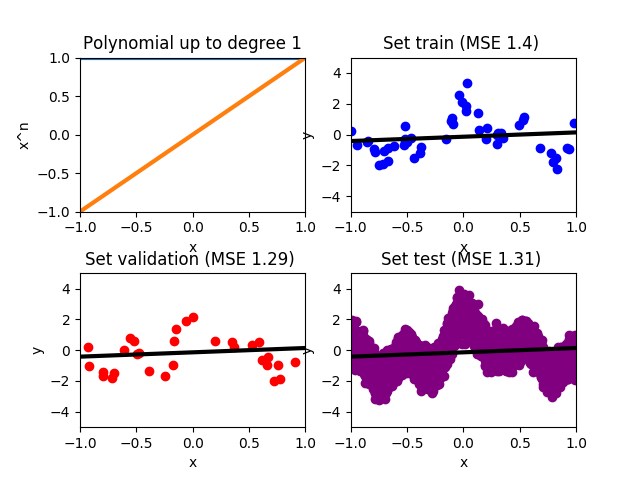
\includegraphics[width=0.5\textwidth]{linreg_deg1.png}%
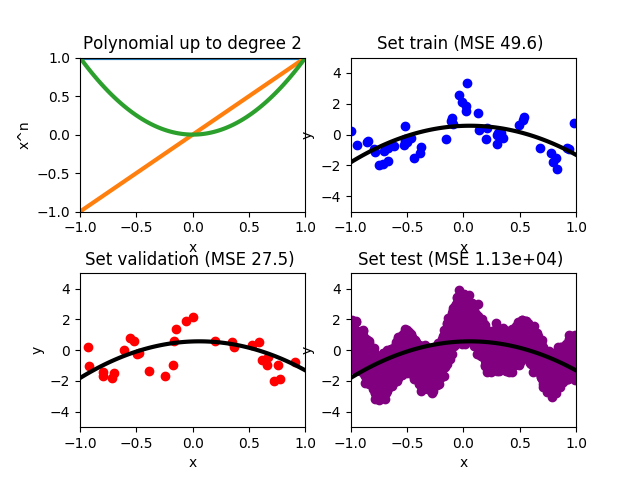
\includegraphics[width=0.5\textwidth]{linreg_deg2.png}\\[2em]
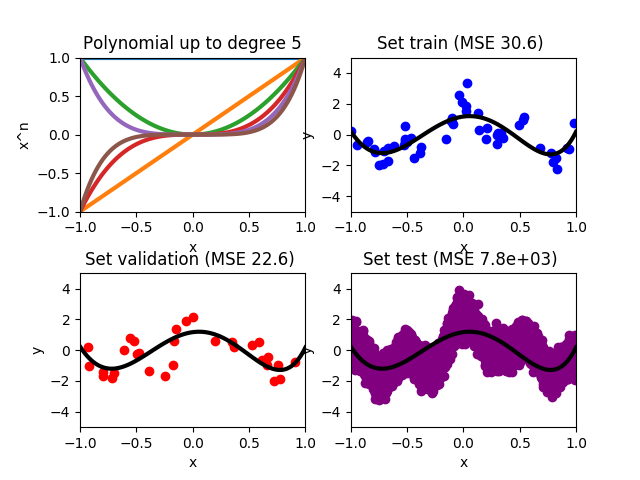
\includegraphics[width=0.5\textwidth]{linreg_deg5.png}%
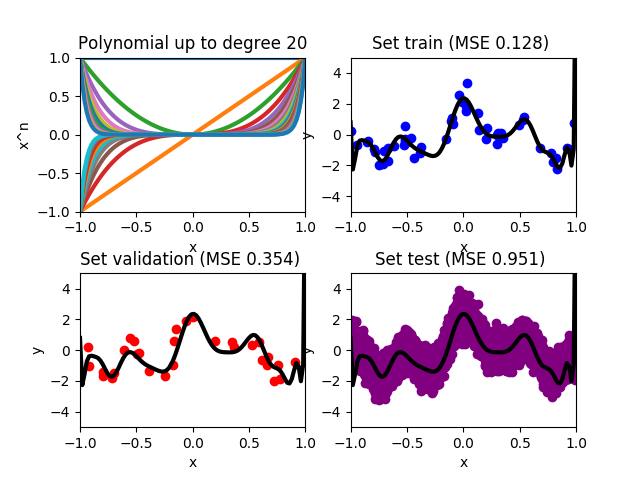
\includegraphics[width=0.5\textwidth]{linreg_deg20.png}\par

\section{Logistic Regression}
\subsection{Derivation of Gradient}
\begin{equation}
\begin{split}
J(\bm{\theta}) &= -\frac{1}{m} \sum_{i=1}^{m} \left( y^{(i)} \log (h_{\bm{\theta}}(\bm{x}^{(i)}))
+ (1-y^{(i)} ) \log (1 - h_{\bm{\theta}}(\bm{x}^{(i)}))  \right) \\
&=  -\frac{1}{m} \sum_{i=1}^{m} \left( y^{(i)} \log (\sigma(\bm{x}^{(i)T}\bm{\theta}))
+ (1-y^{(i)} ) \log (1 - \sigma(\bm{x}^{(i)T}\bm{\theta})  \right)
\end{split}
\end{equation}
The partial derivative of the cost function with respect $\theta_j$ is
\begin{equation}
\begin{split}
\frac{\partial J(\bm{\theta})}{\partial \theta_j }
&= -\frac{1}{m} \sum_{i=1}^m \left(
y^{(i)} \frac{1}{\sigma(\bm{x}^{(i)T}\bm{\theta})} \frac{\partial \sigma(\bm{x}^{(i)T}\bm{\theta})}{\partial \theta_j}
- (1-y^{(i)}) \frac{1}{1-\sigma(\bm{x}^{(i)T}\bm{\theta})} \frac{\partial \sigma(\bm{x}^{(i)T}\bm{\theta})}{\partial \theta_j}
\right) \\
&= -\frac{1}{m} \sum_{i=1}^m \left(
y^{(i)} \frac{\sigma(\bm{x}^{(i)T}\bm{\theta}) \cdot (1 - \sigma(\bm{x}^{(i)T}\bm{\theta}))}{\sigma(\bm{x}^{(i)T}\bm{\theta})} \cdot \frac{\partial \bm{x}^{(i)T}\bm{\theta}}{\partial \theta_j}
 - (1 - y^{(i)}) \frac{\sigma(\bm{x}^{(i)T}\bm{\theta}) \cdot (1 - \sigma(\bm{x}^{(i)T}\bm{\theta}))}{1 - \sigma(\bm{x}^{(i)T}\bm{\theta})} \cdot \frac{\bm{x}^{(i)T}\bm{\theta}}{\partial \theta_j}
\right) \\
&= -\frac{1}{m} \sum_{i=1}^{m} \left(
y^{(i)} \frac{\sigma(\bm{x}^{(i)T}\bm{\theta}) \cdot (1 - \sigma(\bm{x}^{(i)T}\bm{\theta})) \cdot x_j^{(i)}}{\sigma(\bm{x}^{(i)T}\bm{\theta})}
- (1 - y^{(i)}) \frac{\sigma(\bm{x}^{(i)T}\bm{\theta}) \cdot (1 - \sigma(\bm{x}^{(i)T}\bm{\theta})) \cdot x_j^{(i)}}{1 - \sigma(\bm{x}^{(i)T}\bm{\theta})}
\right) \\
&= - \frac{1}{m} \sum_{i=1}^m \left(
y^{(i)} - y^{(i)} \sigma(\bm{x}^{(i)T}\bm{\theta}) + y^{(i)} \sigma(\bm{x}^{(i)T}\bm{\theta}) - \sigma(\bm{x}^{(i)T}\bm{\theta}) \right)\cdot x_j^{(i)} \\
&= -\frac{1}{m} \sum_{i=1}^m \left(
y^{(i)} - \sigma(\bm{x}^{(i)T}\bm{\theta})\right) \cdot x_j^{(i)} \\
&= \frac{1}{m} \sum_{i=1}^m \left( h_{\bm{\theta}}(\bm{x}^{(i)}) - y^{(i)}\right) \cdot x_j^{(i)}
\end{split}
\end{equation}
Thus, the gradient of the cost function is
\begin{equation}
\frac{\partial J(\bm{\theta})}{\partial \theta_j } = \frac{1}{m} \sum_{i=1}^m \left( h_{\bm{\theta}}(\bm{x}^{(i)}) - y^{(i)}\right) \cdot x_j^{(i)}
\end{equation}
\end{document}
